\chapter{Automation}
\label{chap:automation}

\begin{figure}[h]
\begin{tabular}{l r}
\hspace{-1cm}\begin{minipage}{.85\textwidth}
\begin{quote}
{\em The first rule of any technology used in a
business is that automation applied to an efficient
operation will magnify the efficiency.  The second is
that automation applied to an inefficient operation
will magnify the inefficiency.}
-- Bill Gates\index[names]{Gates, Bill}
\end{quote}
\end{minipage}
&

\raisebox{-.8\height}{
	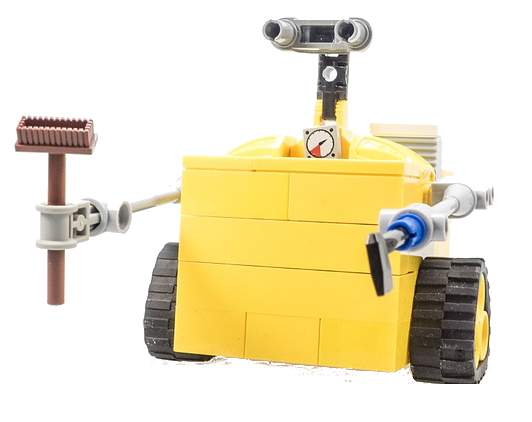
\includegraphics[width=.25\textwidth]{08/pics/wall-e} }

\end{tabular}

\label{fig:wall-e}
\end{figure}

\section{Introduction}
\label{automation:introduction}

In the previous chapter we have discussed how
configuration management systems allow us to create
abstract service definitions and apply the required
changes on the desired sets of hosts.  CM systems thus
remove the need for manual configuration on individual
hosts -- we have automated the steps, and in the
process improved the reliability and scalability of
our services within the infrastructure.

Similarly, we have hinted in Section
\ref{software-installation:os-installation} at systems
capable of performing OS installations across large
numbers of hosts without human intervention.  Knowing
all the individual steps needed to install an
operating system, adding the required software, and
performing initial host configuration (before we
finally let our configuration management engine take
control) allows us to use software to repeat a
previously tedious manual procedure hundreds of times
a day with great ease.

Both of these admittedly complex systems are prime
examples of what system administrators do best: being
inherently ``lazy'' -- a virtue, as we will discuss a
bit more in a minute -- we automate any conceivable
task such that it can be performed at the push of a
button, or perhaps more likely, the press of the
$return$ key.

In this chapter, we will take a small step back
from these large infrastructure components and review
the motivation of the more general concept of
``automation''.  Given the incredible variety of job
descriptions and environments a system administrator
might find herself in, it is not surprising that
the idea of letting computers do our bidding has found
a number of different practical approaches.  We see
evidence of automation as much in a system
administrator's shell aliases or custom scripts as in
the regularly scheduled {\tt cron(8)}\index{\tt
cron(8)} jobs or manually invoked tools.

It has been an old joke that the goal of any great
system administrator is to automate themselves out of
a job, just as we like to suggest to our colleagues or
peers that they should stop bothering us, lest we
replace them with a small shell script.  The use of
this language reflects how we approach automation: our
goal is to not have to perform certain tasks
ourselves, and anything that can be automated, will
be.

Unlike humans, computers do not seem to mind
performing boring, repetitive tasks.  This chapter
looks at how we can take advantage of this fact, how
automation can help you stop wasting your time, and
put to greater use the most valuable resources in any
organization (your engineers' minds). But automation
is no panacea, so we necessarily identify a number of
possible pitfalls and risks as well.

\section{Of Laziness And Other Virtues}
\label{automation:laziness}
\index{Laziness}

System administrators are notoriously lazy.  We don't
want to have to manually swap backup tapes every other
day -- we'd much rather let a robot perform this task.
We don't want to download, extract, build, and install
software packages, hunting down dependencies in the
process -- we'd much rather let our package manager
take care of this.  And we certainly do not want to
sit there all day typing the same set of commands over
and over, when we could instead apply our, in our
humble opinion, significant intellect to solving
mankind's greatest mysteries, such as why the label
maker always runs out of tape in the middle of cabling
a new rack.\footnote{We could, of course, write a quick
script that periodically checks the inventory system
and orders new label maker tape online whenever the
stock supply of label maker tape drops below a given
threshold...}

But being lazy is a virtue -- in this case, anyway.
In order to develop a solution that will save us
tedious work in the long run, we are willing to invest
significant resources up front.  We write scripts that
will take into account a variety of circumstances in
order to allow us to run just one command instead of a
dozen, we schedule checks and implement monitoring
solutions to be notified of events before they become
error conditions, and we write tools that react to
these alerts and which will automatically avert
impending doom.

\AE leen Frisch identified\cite{automation:frisch} --
only slightly tongue-in-cheek -- a number of
``administrative virtues'': Flexibility, Ingenuity,
Attention to Detail, Adherence to Routine,
Persistence, Patience, and Laziness.  While these
traits come into play in almost any of a system
administrator's varied duties, there are particularly
strong parallels to the features that allow us to
create reliable automation tools:

We need {\em flexibility} and {\em ingenuity} to
identify new and perhaps not entirely obvious
solutions to the problems we encounter.

We need to pay {\em attention to detail}, to the
nuances in the ways our systems may differ, when we
analyze and identify all the possible edge cases, or
how invoking a command under certain circumstances can
lead to unexpected results.

We need a strict {\em adherence to routine} to produce
reliable results, to collect usable data, and to keep
our systems maintainable.  We need to follow our own
processes even when we are under pressure and inclined
to take shortcuts, because we trust the routine we
identified earlier more than we trust our stressed out
brains.

We need {\em persistence} and {\em patience} when we write
software, when we debug our tools, when we collect
enough data to be able to identify our outliers and
averages, and we need persistence and patience when we
deploy our new systems, our infrastructure components,
or when we slowly, carefully, replace a much needed
service with different software.

But what impacts most of our practical work turns out
to be {\em laziness}.  As soon as we run a lengthy command a
second or third time, or as we repeat a series of
complex steps to complete a specific task, we start to
wonder how we can script this.  Sure, we may end up
spending a lot of time getting our automated jobs just
right, but we gain productivity in the long run.  And
so our laziness pays off.

\section{Benefits of Automation}
\label{automation:benefits}

When we look at large infrastructure components that
help automate a complex process or workflow such as
the deployment of a new host, it is immediately
obvious that we reap significant benefits from having
developed such a system.  But even on a much smaller
scale do we discover the same advantages, even though
we may initially begin the process of automating a
given task with the only goal being to save ourselves
some typing.  The primary benefits we derive from
implementing an automated solution -- even in the
small -- include the following.

\subsection{Repeatability}
\label{automation:benefits:repeatability}

Typing the same set of commands over and over is
tedious.  A few years ago, while maintaining a
heterogenous environment of NetBSD/i386 and IRIX/mips
systems, I had to try to keep in sync the latest
version of the \gls{gcc}\index{\tt gcc(1)},
standardizing it to fit into our environment, enabling
only the required languages but at the same time
ensuring the build of a 64-bit binary\footnote{Certain
64-bit capable IRIX systems supported both a 32-bit
and a 64-bit \gls{abi}\index{Application Binary
Interface}; in order to use the more performant 64-bit
interface, the application would have to be compiled
with support for and be linked against the 64-bit
libraries.  Even though less common today, you can
still find a number of tools that cannot (easily) be
built as 64-bit binaries.}.

Normally, you would have your package manager perform
this installation.  However, as discussed in Section
\ref{software-installation:package-management:manual},
there are situations where installing software ``by
hand'' is your only option.  This was one of them: the
native package manager did not provide a 64-bit
version of this compiler, and what might otherwise
seem like a routine task -- building a new compiler --
required the setting of a number of environment
variables and command-line options to the {\tt
./configure} script.  In order not to have to remember
all the right settings, I wrote myself a trivial
script (see Listing \ref{code:automation:gcc}.

\begin{lstlisting}[float,label=code:automation:gcc,caption={[Script
to build GCC on an old IRIX system]Building a 64-bit
version of the GNU Compiler Collection on an old IRIX
system. Even if done rarely, storing these commands in
a rudimentary script can help repeat the process more
easily. (With plenty of room for improvement, Problem
\ref{prob:automation:improve-script} will ask you to
turn this into a more reliable, more readable tool.)}]
#! /bin/sh
export CC=cc CXX=CC CFLAGS="-64 -mips4 -r10000" LDFLAGS="-64"
mkdir gcc-build
cd gcc-build
../gcc-3.3.3/configure --prefix=/usr/pkg/gcc-3.3.3         \
        --enable-languages=c,c++,java --enable-libgcj      \
        --disable-shared --enable-threads=posix            \
        --enable-version-specific-runtime-libs             \
        --enable-haifa --disable-c-mbchar                  \
        --disable-checking --disable-nls
gmake bootstrap
\end{lstlisting}

A few months later, when a new version of
\verb+gcc(1)+ became available, I had to repeat the
same process.  Instead of wasting time trying to
remember all the options I needed, what environment
variables I had to set, etc., I was able to build it
using this trivial script.

We often use automation as a way to remember the
correct steps.  Even a task that is not performed
frequently -- in our example above, perhaps twice a
year -- benefits from us creating even a simple script
to repeat it easily without having to think twice
about every detail.  Detailed documentation explaining
{\em why} certain parameters need to be passed may be
ideal, but providing a simple script to repeat a
cumbersome process is still a win.

Guaranteed repeatability allows us to ignore {\em how}
a task is performed.  Even simple scripts can thus
hide unnecessary complexity from us, making the task
at hand easier in the process.

\subsection{Reliability}
\label{automation:benefits:reliability}

Being able to repeat the same process easily without
having to recall the details of every step is a great
advantage, not only because it saves us a lot of
typing or because we don't waste time recreating
previously known information.  One of the key benefits
of an easily repeatable process lies in its {\em
reliability}.  When we run commands interactively, we
may change the order or detail of invocation as we run
through the end-to-end process.  We easily make
mistakes, mistype a command, accidentally redirect
output to truncate a file instead of appending to it,
accidentally slip in an additional character, execute
a command from the wrong directory, or we simply skip
a step (by accident or because we deem it
unnecessary).

Every time we invoke a script, on the other hand, it
will run the same commands in the same order.  If we
are careful when we automate a task and create a tool
executing idempotent commands only (hopefully combined
with copious error checking), we need not worry about
how it is invoked.  We can treat it like any other
system utility and rely on it running either to
completion or produce meaningful error messages that
allow us to diagnose the problem.

Automation provides reliability not only through
consistency, but also in terms of quality: as soon as
we begin to automate a task, we begin to move beyond
just stashing individual commands in a script (such as
the one given as an example above).  Instead, we build
our tool with reliability in mind, fine tuning the
steps and beginning to think more about how they are
executed.  Just like documentation, we are more likely
to consider in more detail the implications of each
command when we create an automated job.  As a result,
the final utility is more robust and executes more
reliably than any manual process ever would.

Some tasks need to be performed repeatedly with a
certain regularity, system backups being a prime example.
For starters, the backup process needs to be
run on a daily basis.  Defining the command required
to initiate this task and then scheduling it via the
{\tt cron(8)} d\ae mon is about as mundane yet
important a task as you may encounter in any system
administrator's life.  But being able to rely on the
tool is a pre-requisite, and automating the steps to
allow them to be scheduled in the first place does
provide this required reliability.

\begin{experience}
{\bf Robots to the rescue!} \\

Automation can not only be achieved by scripting or
programming.  Several years ago, it was not uncommon
for small sites to use a single tape
library\index{tape library}, storing backups on a
rotating set of backup tapes.  This meant having to
change the tape on a daily basis, as otherwise you
would overwrite the previous day's backup.  It turns
out that most humans are fairly bad at remembering
such tasks -- at one time, I had the backup system
email me a daily reminder in the afternoon to rotate
the tapes; I still forgot to do it every now and then.
\\ [10pt]

As our systems grew and disk capacity increased, so
did the requirements for backups.  Eventually,
upgrading our backup system became unavoidable.  At
that point, we invested into a significantly larger
(albeit substantially more expensive) tape library able
to hold dozens of backup tapes and to rotate them
automatically by means of an internal robotic tape
switcher.  \\ [10pt]

Once set up correctly, the entire backup process
became completely automated, not requiring any human
intervention whatsoever.  Every so often, ``throwing
money at the problem'' may turn out to be the best
solution.  The satisfaction of seeing a robot do one's
manual work should also not be underestimated.  But
all automation solutions, including robots, can
experience unexpected failures.  At Yahoo!, we once
received an incident notification that read: ``Two
robots collided, one arm pulled off.'' Fortunately,
the appendage in question belonged to one of the
robots, not a datacenter technician.  \end{experience}


\subsection{Flexibility}
\label{automation:benefits:flexibility}

As we develop our tool, it often becomes obvious that
we are not, as initially assumed, solving one specific
problem, but that we are facing a particular instance
of an often more generic set of problems.  In our
previous example, we set out to build a script that
would let us easily create a 64-bit version of version
3.3.3 of the \verb+gcc(1)+ tools.  We hard-coded both
the \gls{abi} as well as the software version into our
simplistic script, meaning that the next time a new
version is released, we need to edit the source to
build the software.  What's more, some of our machines
do {\em not} support the 64-bit \gls{abi}, and we need
to build 32-bit versions as well.  In other words: we
need a more flexible tool that allows us to specify
both the ABI as well as the software version.

%\begin{lstlisting}[float=ht,label=code:automation:gcc-script,caption={[A
%second iteration of our {\tt gcc(1)} building
%utility]A second iteration of our {\tt gcc(1)}
%building utility, showing some added error checking
%and increased flexibility through the use of
%command-line options.  Our tools often evolve in this
%manner from a trivial script into a more functional
%program.}]
%#! /bin/sh
%set -e
%
%VERSION="${1:?"Usage: ${0} <version> [abi]"}"
%ABI="${2:-64}"
%DIR="${TMPDIR:-/tmp}/gcc-build"
%
%export CC=cc CXX=CC CFLAGS="-${ABI} -mips4 -r10000" LDFLAGS="-${ABI}"
%
%mkdir -p "${DIR}"
%cd "${DIR}"
%
%if [ ! -d "${TMPDIR:-/tmp}/gcc-${VERSION}" ]; then
%        echo "GCC source dir not found." >&2
%        exit 1
%fi
%
%../gcc-${VERSION}/configure --prefix=/usr/pkg/gcc-${VERSION}\
%       --disable-c-mbchar                                   \
%       --disable-checking                                   \
%       --disable-nls                                        \
%       --disable-shared                                     \
%       --enable-haifa                                       \
%       --enable-languages=c,c++,java                        \
%       --enable-libgcj                                      \
%       --enable-threads=posix                               \
%       --enable-version-specific-runtime-libs
%
%gmake bootstrap
%\end{lstlisting}

Once identified as a candidate for automation, we
quickly begin to view the problem at hand in a
different context.  By spending a little bit of time
up front, we can anticipate future requirements and
make our tool useful in a variety of circumstances.
For example, we may allow the user to specify
different options on the command-line or let the tool
react to certain environment variables.

But flexibility is not only exhibited by allowing
different invocations.  A good tool is also flexible
in the way in which it handles certain error
conditions.  This may be achieved by verifying any of
the assumptions made, or by failing early and
explicitly.  This behaviour reflects the concepts of
{\em Idempotence}\index{idempotence} and {\em
Convergence}\index{convergence}, which we discussed in
Chapter \ref{chap:configuration-management}; we will
go back to these and other desirable features of
scalable tools in Chapter
\ref{chap:building-scalable-tools}.  For now, suffice
it to say that even if somewhat paradoxically a tool
being more strict about how it runs may actually
provide greater flexibility: it allows us to run it
under different circumstances with predictable
outcomes.  What's more important: it may allow us to
build other tools {\em around} it.

%Take a look at Listing
%\ref{code:automation:gcc-script}, where we have added
%some error checking as well as options to build either
%32-bit or 64-bit binaries of the specified version to
%our simple example script.  While there is still
%plenty of room for improvement (part of Problem
%\ref{prob:automation:improve-script}), we increased
%both the reliability and flexibility of what started
%out as a collection of fixed commands stashed away in
%a file.

\section{Who benefits from automation?}
\label{automation:who-benefits}

The evolution of individual, trivial scripts into more
generally useful utilities and tools is inevitable,
and one of the key benefits of committing to
automation of your routine tasks early on.  Frequently
we start out just trying to save ourselves a few
keystrokes and end up writing a program which many
other people rely on for their day to day work.
Figure \ref{fig:automation:tools-evolution}
illustrates this evolution of system administrators'
tools from e.g. a shell alias into a full-fledged
service or widely used tool.  Note that the more
mature your tool becomes, the more likely it is that
others have begun customizing it or written scripts
that depend on it.  This implies a stability
requirement in more mature tools: the more users
depend on it, the harder it is to make significant
changes.

It is thus a good idea to remember who we are
automating a task for, as that helps us define exactly
how to shape our tools.  Broadly speaking, we often
automate tasks for ourselves, for our peers (other
system administrators within or outside of our
organization), and finally for other users in general.
As the number of possible users of our tools in these
three groups increases, the number of assumptions we
can safely make about how the tool is used, or the
environment in which it runs, goes down.

Each category exposes significantly different inherent
complexity, but the resulting benefits tend to
increase as well.  Much as with documentation, as we
discussed in Chapter \ref{chap:documentation}, clearly
identifying your target audience (or user base in this
case) is an important prerequisite to building a new
automation solution.

\subsection{Ourselves}
\label{automation:who-benefits:ourselves}

Often we begin automating a task by customizing our
own environment.  We all have our own shell aliases,
functions, or custom little scripts stored in our home
directory or a private location in our {\tt PATH}.

The script we used in the previous section is a
good example:  we did not anticipate anybody else to
have to perform this task, and so we took the liberty
of making a few assumptions about the environment in
which it might be executed.

As system administrators, we should be careful not to
create tools that only benefit ourselves, as this
approach does not scale well.  In any but the smallest
organizations, we share responsibilities with others
and operate in sufficiently diverse environments to
not be able to rely on too many customizations.

It is not uncommon for senior system administrators in
large organizations to have the most bare-bones shell
startup files of all users, despite being the perhaps
most advanced users.  Not relying on assumptions about
and customizations of the shell environment is
something learned and appreciated with experience.  In
fact, just being consciously {\em aware} of the
assumptions we make is often a sign of a senior system
administrator.

\subsection{Our Peers}
\label{automation:who-benefits:peers}

Even the little scripts we create for ourselves tend
to evolve into larger programs as we share them with
our peers.  As the number of users increases, so do
the requirements.  We need to start to accommodate
different use cases and different environments.

In many organizations, system administrators create
their own tools to automate every conceivable task of
their daily routine.  In larger environments, this may
become a specialization of some members of the
sysadmin team, and yet others may even provide a team
dedicated to the development of these tools.

If you work in a small environment, try to think
within the context of a significantly larger scale
about the various tasks you perform and have
undoubtedly automated for yourself.  If you work in a
large environment, try to think how the many tools you
use regularly have evolved.  One of the key
differences in these two points of view is the target
audience.

Also note that developing tools for system
administrators to automate their very specific and
often complex tasks requires a very specific
background.  System administrators are power users,
who have high expectations of their tools; we tend
to quickly dismiss anything that does not meet them.

\begin{figure}[!t]
	\centering
	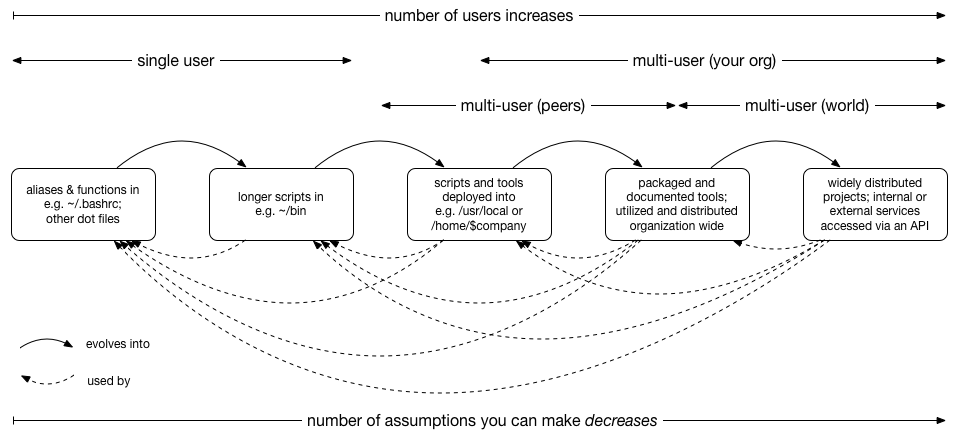
\includegraphics[width=0.95\textwidth]{08/pics/tools-evolution}
		\caption[Evolution of SysAdmin Tools]{
			SysAdmin tools often evolve with time.
			Complexity increases with the
			number of users, while the
			number of assumptions you can
			safely make about the
			environment in which the tool
			is invoked decreases.
			\label{fig:automation:tools-evolution}}
\end{figure}


\subsection{All Users}
\label{automation:who-benefits:all-users}

Recall from the introductory chapter of this book that
one of the definitions of a system administrator is
``one who, as a primary job function, manages computer
and network systems {\em on behalf of another}.'' The
main reason for the systems we maintain to exist is so
they can perform a specific service.  That is, their
purpose implies a number of users who take advantage
of the system's resources.  These users may be actual
user accounts on the systems or external users
interacting with the systems over the network.

In order to allow our users to get the most out of our
systems, we frequently put together tools that
automate common tasks or interactions on behalf of all
users.  This may be a simple tool to allow a user to
retrieve or request one of their files from backup, a
program to facilitate access to an internal database,
or perhaps a utility to let users receive system or
software updates.

As we develop these tools, we need to keep in mind the
requirements of the user interface, as well as --
again -- what assumptions we make about the user's
environment and even abilities.  It is also worth
noting that, depending on the size of the environment
you work in, the difference between automating a
system administrative task and developing a large
infrastructure service quickly become rather fuzzy.  As
noted above, in some organizations, dedicated teams
are created to provide and maintain custom tools for
use in the administration of the systems.  Some of
these tools are open sourced and distributed outside
of the company, yielding a massively increased user
base.

\section{Levels of Automation}
\label{automation:levels}

Automation is a term with many different meanings.
Within System Administration, we often encounter a
mantra that any conceivable task, if repeated only
twice, should be automated.  But the outcomes and
level of effort required vary significantly depending
on exactly how far we want to take this approach.
Earlier, we cited the examples of Host Deployment and
Configuration Management to illustrate what it means
to automate a very complex task from end to end;
throughout this chapter, we have used a much simpler
example to show how we may also benefit quickly from
trivial automation.

As we can see, there are obvious differences in the
level to which we may take automation.  Writing a
small script to avoid having to repeat the same tasks
is perhaps the simplest version of automation, yet it
often evolves into a more complex solution, expanding
with the problem scope.  After completing a task, we
often realize that it was just one step of a longer
process, and that we may well automate the remaining
steps as well.

Automation is rarely completely autonomous.  By this,
we mean that we define specific subsets of tasks that
are performed by a computer on our behalf, but the
overall operation, divided into answering questions
about the {\em what}, {\em how}, {\em when}, and,
ultimately, {\em why} of a given problem solution, are
to be answered by the system administrators in charge.

Tools written to save typing efforts, even if they
include logic that provides flexibility to yield
different outcomes depending on certain circumstances,
by and large provide answers to the question of {\em
how} to solve a problem by having a human describe
detailed instructions.  That is, we describe the steps
necessary to be executed in their specific order.  In
our previous example, we identified the goal of the
tool (``Build a new version of the \verb+gcc(1)+
compiler.'') and provided a script describing the
method of accomplishing it (``Set these environment
variables.  Run the \verb+configure+ script with these
options.  Run the \verb+make+ command.'').

The level of automation reached here is fairly low,
but it has the advantage that the solution is simple.
As we move beyond this first stage of automation, we
begin to define the problem in more general terms,
allowing us to describe only {\em what} we wish to
accomplish without having to care about {\em how} this
is done.  In our example, a generic package manager
might serve as the automated solution: we can specify
that we need a new version of a package, without
having to know (or care!) about how the system
actually builds it.  Despite increased complexity, the
benefits are significant.  In addition, we still
control {\em when} actions are taken interactively.

Configuration management takes automation to the next
level: here, system administrators only describe the
{\em what}: which packages should be installed, which
files should be added, updated, or removed, etc.,
without always specifying exactly {\em how} this is
done, nor {\em when} these steps are to be
executed.\footnote{To be fair, writing the rules of a
configuration management system may frequently include
a specification of the {\em how}, but with sufficient
abstraction, such as by way of carefully crafted
templates, these details become less important for
routine configuration tasks.} That is, the
configuration management system is more autonomous, as
it applies its own rules of which steps to perform at
what time to yield eventual convergence to the defined
state.

Similarly, monitoring tools that trigger actions based
on pre-defined thresholds or events are a way to
automate the {\em what} and {\em when} of some system
recovery tasks, but they may leave the {\em how} to
either humans (in the case of alerting) or another
system.  As we combine these different levels of
automation, we can -- sometimes -- approach the golden
grail of system administration: autonomous,
self-healing systems.  At this stage, the software
decides on its own what actions to perform based on
the input of its various subsystems or components.  It
may still inform its system administrators of the
steps executed, but no longer require human
interaction for the majority of events.  In some
cases, there is even hope to allow systems to become
more adaptive and to execute different steps based on
data collected from previous instances of the same
event -- it may ``learn''.

The thought of self-adapting, autonomous computers
managing large systems without human interaction may
sound futuristic or even a bit concerning, and it
carries significant risks: at each step, complexity
increases manifold, and the opportunities for
catastrophic failures may indeed multiply.  We discuss
some of these disadvantages in the next section.

\section{Automation Pitfalls}
\label{automation:pitfalls}

So far we have praised automation for all its
benefits: increased reliability, flexibility, for
allowing us to schedule tasks and then -- for the most
part, anyway -- forget about them, knowing that they
will run and Do The Right Thing.  But automation is no
panacea; as so many things in life, it involves
trade-offs.

Most obviously, taking a complex task and defining it
in such a way that it can be automated requires a
thorough understanding of the problem and its possible
pitfalls, of any possible side-effect, how much
variance your environment exhibits, and how much you
wish to be able to accommodate with the automated
solution.  This is still a {\em benefit} of
automation, as you begin to more clearly understand
the problem space, and are more likely to identify a
more reliable solution.

But performing this analysis and then implementing
(and debugging!) the tools to automate the task at
hand takes time and effort.  In addition, one needs to
remain aware that applying the results of our
automation efforts to build further tools may trap us
in what is known as ``confirmation bias''\index{Bias,
Confirmation}: as we measure what we can, we may
erroneously dismiss what we could not or did not
measure.  Trusting our automated tools can lead us to
overlook or dismiss factors not accounted for in these
solutions.  We will take a closer look at this effect
and related risks when we discuss monitoring in more
detail in Chapter \ref{chap:monitoring}.

\subsection{Increased Complexity and Impact}
\label{automation:pitfalls:complexity}

Automation often introduces or increases complexity.
Unless carefully implemented and meticulously
documented, an automated system can become a black box
to your peers.  Fewer people will understand how the
task is actually accomplished or where to look when
things inevitably break.  ``Complex systems fail in
complex ways.''\cite{automation:cook}

Automation also vastly increases the impact of any
failure you may encounter, as it allows us to perform
tasks across the entire infrastructure.  While a
manually executed command may well be mistyped, it
will often have a limited impact.  After all, this is
often precisely {\em why} we wanted to automate the
given task!  But now consider the failure scenario:
accidentally removing a user account from a single
machine, for example, is easy to fix and may not
impact that system's operations; accidentally removing
all user group associations from all of your
infrastructure's hosts, on the other hand, may cause
wide spread system failure and be much harder to
revert.

Well-written tools prevent such catastrophic failures
-- or at least, they will try to.  But at the end of
the day, these tools are written by ever-fallible
humans, and so bugs sneak in.  A simple typo in a
wide-spread tool can wreak havoc on an impressive
scale.

\begin{sidenote}
{\bf The Impact of a Single Character} \\

Software installation and upgrades are frequently
automated (whether by way of a package manager or a
{\tt Makefile}) using simple scripts that perform the
necessary steps.  For example, a package owning the
files under the {\tt /usr/lib/mumble} directory might
delete those files when it is upgraded or removed. \\
[10pt]

In 2011, users of a specific software package noticed
that upgrading from one version to another rendered
their system completely unusable.  Looking at the
install script of the software, it was found to
contain the following command: \\ [10pt]

\verb+rm -fr /usr /lib/mumble+ \\ [10pt]

If you look closely, you will notice that there is an
erroneous space between the {\tt /usr} and {\tt
/lib/mumble} components of the pathname.  The package
had intended to remove only the subdirectory
containing files it previously installed, but
proceeded to recursively remove all files under {\tt
/usr}, a critical and sizeable part of the operating
system! \\ [10pt]

Recall from Section
\ref{software-installation:package-management:security-risks}
the inherent risk of trusting your package manager (or
any third-party software whose install scripts you run
with superuser privileges without careful inspection)
-- this example helps illustrate that point as well as
the possible impact a single character in the wrong
place may have. \\ [10pt]

Even though this particular error was quickly detected
and fixed, imagine your automated software deployment
system pushed an upgrade of this specific package to
all of your hosts, and you will quickly understand how
automation can magnify any failure exponentially.
\end{sidenote}

\subsection{Loss of Audit Trail}
\label{automation:pitfalls:audit}

Any but the most simple of infrastructures requires
operations on a number of different resources:
information about host groups are stored in and
accessed from one database, subsets of hosts are
accessed in order to manipulate resources in another
segregated access zone, and so on.  For human
interactions, all of these actions are (hopefully)
explicitly authenticated and logged, allowing us to
track who initiated what changes where and when.

When we add automation into the mix, we frequently
have to create a so-called ``service account'', an
account that is not associated with a person, but that
exists to allow automated tools to perform certain
actions.  We noted in Section \ref{multi-user:types}
that the mapping of real people to user accounts is
neither subjective nor bijective; these service
accounts are but one example thereof.

Odds are that a fictional company named ``Weeble''
does in fact have a Unix user-ID ``weeble'' on
virtually every single host, which is likely used for
software deployment or system administrative tasks.
Many automated solutions will use this account to
access systems or internal resources, and even though
considered an ``unprivileged'' account, it probably
has sufficient access permissions to cause significant
damage.  What's more, it's unlikely that actions by
this user can (easily) be tracked back to a human, an
important auditability requirement.

In this case, the ability to orchestrate complex
changes across large sets of hosts may lead to a loss
of the audit trail.  Granted, it is possible to retain
the ability to track commands and actions, but even
when that is not flat out neglected, with every added
level of automation this becomes more and more
cumbersome.  Identifying who specifically initiated a
chain of events, and ascertaining whether the correct
access was applied becomes increasingly difficult.

\subsection{Loss of Accountability}
\label{automation:pitfalls:accountability}

Even if we may not be able to track every single
command executed by any automated system, we need to
be able to identify on a higher level what changes
were {\em initiated} by whom.  In today's massive
infrastructures, automated systems make decisions
about which servers to shut down, which ones to direct
production traffic to, or which IP addresses or
networks to automatically block.  These decisions are
made automatically, based on traffic patterns, system
monitoring, and a number of other factors.

While we need to allow for this level of automation in
order to meet the rapidly rising demands on our
infrastructure, we {\em also} have a conflicting
requirement of accountability.  Every action performed
on our systems need not be tied directly to a human,
but the decision engine that automatically applies the
given heuristics needs to regularly be reviewed and
allow for an audit trail.

Remember: due to the ease with which our automated
tools allow us to administer large numbers of
machines, the size and impact of any outages will be
significantly increased as well!  Untangling the web
of decisions made that led to a system wide outage
becomes harder and harder due to the increased
complexity of both the run-time systems as well as
the failure modes.  In the end, we need to be able to
identify exactly {\em why} the system failed in the
way that it did.  What was the {\em root
cause}\index{Root Cause Analysis}?\footnote{It turns
out that trying to pinpoint failures to a {\em single}
``root cause'' is often overly simplistic.  A more
thorough understanding of how complex systems
interact, and how human decision making processes
contribute and may be built into such systems is
becoming an interesting field of study all by
itself.  Look for works by
Allspaw\index[names]{Allspaw, John},
Cook\index[names]{Cook, Richard},
Dekker\index[names]{Dekker, Sydney} et al on the topic
of Root Cause Analysis and ``Human Error''.}

Similarly, from a security perspective, it is
imperative to be able to tell who initiated a certain
action -- not in order to ``blame'' that person for
causing an outage, but to be able to identify a
possibly compromised account or e.g. overly broad access
permissions.  Government issued
guidelines or regulations
%, such as the {\em Payment Card Industry Data
%Security Standard} (\inx{PCI DSS}),
may require your organization by law to be able to
provide a full audit trail of certain actions.  With
the help of automation, we can actually improve our
auditability and accountability, but these factors do
need to be considered and integrated into the tool or
product right from the beginning.

\subsection{Safeguards}
\label{automation:pitfalls:safeguards}

The complexity we inherit as a by-product of all the
benefits of automation should not be underestimated.
With every additional automated step, we broaden the
possible impact of our tool.  Not only can more things
go wrong, but failure may propagate or escalate at
scale.  As a result, the need for safeguards together
with the discovery of and alerting on error conditions
increases at the same rate.

Simple tools rarely require human interaction, but may
at times allow for confirmation from the user before
taking a particular action; as an example, consider
the {\tt -i} flag to the {\tt cp(1)}, {\tt mv(1)}, and
{\tt rm(1)} utilities.  As we combine such tools (or
write our own) to provide more automation, such
safeguards are often seen as a hinderance, and we
avoid them where possible.  After all, the whole point
of automating a task is to avoid human interactions.
But as we do so, we also increase the risk of more
widespread damage when (not {\em if}!) things do go awry.
Smart tools make use of well-defined thresholds when
applying large changes: a tool may allow you to update
or delete records in your inventory database without
interaction (assuming proper authentication), but may
ask for additional confirmation or even higher
privileges when performing the same action on {\em
all} records.

\begin{sidenote}
{\bf Lessons from an Amazon Service Outage} \\

On Christmas Eve 2012, Amazon suffered a major outage
of their ``Elastic Load Balancing'' (ELB)
service\cite{automation:aws-outage}.  A significant
amount of state data tracking which hosts should
receive traffic was accidentally deleted from the load
balancers in Amazon's largest region.  This event had
a cascading effect that was particularly disastrous
for one of Amazon's biggest \gls{aws} clients,
Netflix, on a day when traffic is expected to be at
peak times. \\ [10pt]

The root cause of this outage was, as so often,
determined to be ``human error'': developers
accidentally initiated data deletion commands against
the production- instead of their maintenance
infrastructure.  The effects of this action trickled
down to each customer, leading to confusing \gls{api}
errors in the service.  It took Amazon several hours
to fully understand why the errors occurred and before
a restoration of the service could even be attempted.
Given the complexity and size of the infrastructure at
hand, this is not very surprising. \\ [10pt]

%What is particularly interesting in this case is that
%up to this point Amazon's engineers appear to have
%been able to make such large changes affecting
%production services without explicit Change Management
%approval.  As a direct result of this outage, Amazon
%then suggested that in the future Amazon will require
%developers to seek explicit approval for similar
%changes.  What was, presumably, an agile and mostly
%automated mechanism now appears to have become a
%procedure that requires multiple interactive steps
%during which different people in an organization have
%to review and approve the changes. \\ [10pt]

We can see a number of parallels to the pitfalls of
automation we have discussed. First, the complexity of
the systems meant that engineers spent hours
troubleshooting the failures, slowly tracing cause and
effect back to human initiated actions. Second, the
impact of the changes applied by the developers was
magnified by multiple layers of automation, and not
limited to Amazon themselves: many of Amazon's
customers were directly affected (in dramatic ways),
and had no, or only limited, means to mitigate their
losses.  Finally, missing safeguards allowed the
changes to be applied without required approval.
\end{sidenote}


Since it is always easy to identify in hindsight the
parts where our tools should have had safeguards it is
not uncommon to encounter such safety measures only
after an undesirable incident has occurred.  This is
not surprising: our tools evolve with time, and what
is obviously necessary in a large scale solution is
easy to dismiss as overhead in a simple script.  But
at the same time, adding safeguards, error-checking,
privilege separation, logging, event correlation, and
monitoring is so much easier to do when developing a
small tool; refactoring a complex system already in
production use to add these essential features is
significantly harder.  This is why it is important to
be aware of the possible pitfalls of automation right
from the start.  We need to build our tools in a
scalable manner and with the foresight and
understanding that they may well evolve into a much
larger service or component of a bigger solution.

Yet we need to be careful not to hamper productivity
with pointless requirements for human interactions:
requiring sign-off by a peer or supervisor before
issuing routine commands is not only demotivating and
tedious, it becomes unsafe when users find ways around
the restrictions.  Any safeguard that users do not
understand, or that ultimately get in the way of them
getting their job done, will eventually be
circumvented.  We will revisit this dilemma when we
discuss general security principles in Chapter
\ref{chap:security}, but the question how, when and
where to add the necessary safeguards without
impacting effectiveness remains one of the fundamental
conflicts when developing an automated solution.

\section{Summary}
\label{automation:summary}

Automation is an essential part of every system
administrator's life.  We encounter it on a daily
basis in small tools as well as in large and complex
infrastructure components.  We noted, half
jokingly, that laziness is an inherent trait, a
virtue, of every good system administrator, which
paradoxically may lead us to go to great lengths and
significant efforts to have computers perform the
tasks we would otherwise need to repeat ourselves.

We have looked at the explicit benefits automation of
even trivial tasks provides: we gain the ability to
repeat complex command invocations without having to
remember all required options or environment settings;
we begin to rely on our tools as they grow and allow
us to ignore the implementation details, knowing that
a carefully written script or program can be trusted
to perform the right sequence of steps;  we gain
flexibility in the execution of many tasks as we apply
some abstraction and build tools that solve not just
one specific problem, but allow us to address more
general classes of problems.

Parallel to these benefits, we noted that different
users benefit in different ways from the tools we
create.  Just as we increase flexibility through
abstraction, so do we improve the usefulness of our
tool as its userbase grows.  But automating
administrative tasks for all users of our systems or
our peers requires a different understanding of the
problem space than if we were merely jotting down a
quick script to help ourselves save a few keystrokes.
As with documentation, we need to understand our
target audience.

As we began to realize that even our simple example
script has already started to show signs of evolving
into a larger solution, we noted the different levels
of automation.  The more advanced the system, the more
autonomously the computer makes decisions and issues
commands, the higher the degree of automation.  At the
lowest level we find a simple, human provided
description of individual steps of {\em how} to reach
a desired outcome.  The larger and more abstract
question of {\em what} we wish to accomplish is
initially outside our scope, but quickly becomes the
central goal as we grow our initial tool into a more
generally useful application.

We cited automated deployment and configuration
management systems as examples of a high degree of
automation.  In some of these cases, we need only
state the abstract goal, allowing the computer to
decide autonomously which steps are necessary to
execute as well as when to execute them.

As these systems grow more complex, they become more
autonomous and powerful.  As noted by John
Allspaw\index[names]{Allspaw, John}, the value of
automation ``is extremely context-specific,
domain-specific, and
implementation-specific''\cite{automation:allspaw}.
It is therefor important for us to be acutely aware of
the specific needs which a given solution was designed
to meet as well as the many risks associated with
increased levels of automation.  The benefits
automation may provide come at a (non-negligible)
cost; automation for automation's sake is risky.

We looked at the possible downsides or pitfalls of
automation and identified within this context the
increased complexity, repeatedly called out as our
nemesis throughout this book, and impact of any
possible failure, the possible loss of auditability
and accountability, as well as the greater need for
safeguards.  As system administrators, we have to be
aware of the explicit -- and more often: implicit --
trade-offs we make as we apply or create automated
solutions.  In the next chapter, we will take these
lessons and attempt to turn them into more concrete,
practical advice for developing scalable tools.

\vfill
\pagebreak

\chapter*{Problems and Exercises}
\addcontentsline{toc}{chapter}{Problems and Exercises}
\section*{Problems}
\addcontentsline{toc}{section}{Problems}

\begin{enumerate}

\item
\label{prob:automation:frequently-used}
Take a look at your shell's history file, e.g. {\tt
\~{}/.bash\_history}.  Which commands do you run most
frequently?  Can you create aliases or shell functions
that save you some typing?

\item
\label{prob:automation:routine}
Identify a routine task you perform on a regular
basis.  How can you automate this task?  Can it be
broken into smaller independent subtasks that can be
automated?

\item
Ask your peers, your local system administrators, or
search the Internet for examples of simple scripts and
custom tools they use.  How flexible are these tools?
What assumptions do they make about their environment?
Can you improve one of them?

\item
\label{prob:automation:improve-script}
Consider the example script from Listing
\ref{code:automation:gcc}.  What assumptions
does it make?  How would you change the script to
improve its reliability and flexibility?

\item
Review the exercises
\ref{prob:software-installation:pkg-vs-manual} and
\ref{prob:software-installation:build-a-package} from
Chapter \ref{chap:software-installation}.  What kind
of automation do the different package managers
provide?  What kind can/did you apply in solving the
problems?

\item
Identify the methods by which your systems are
maintained and updated, including the configuration
management, software deployment and service monitoring
systems.  Which steps are performed manually?  What
level of automation can you identify?

\item
Search the Internet for a recent, significant service
outage.  What did you learn about the root cause of
the failure?  What role did automation play?  What
kinds of safeguards were triggered, missed, or added
after the fact?

\item
Think about automation outside the context of system
administration.  Do the same principles we discussed
here still apply?  Can you identify different levels
of automation or its pitfalls in the so-called ``real
life''?

\end{enumerate}

\vfill
\pagebreak

\bibliographystyle{plainnat}
\begin{thebibliography}{99}

\bibitem{automation:frisch} \AE leen Frisch, {\em Essential System
Administration}, O'Reilly Media, 2002

\bibitem{automation:ironies} Lisanne Bainbridge, ``Ironies of
Automation'', {\em Automatica}, Vol. 19, No. 6, Pergamon Press Ltd. 1983;
on the Internet at \\
{\url http://www.bainbrdg.demon.co.uk/Papers/Ironies.html} (visited April
1st, 2013)

\bibitem{automation:woords} David D. Woods, ``Decomposing Automation:
Apparent Simplicity, Real Complexity'', {\em Automation and Human Performance:
Theory and Applications}, CRC Press, 1996.

\bibitem{automation:allspaw} John Allspaw, ``A Mature Role for
Automation: Part I'', on the Internet at \\
{\url
http://www.kitchensoap.com/2012/09/21/a-mature-role-for-automation-part-i/}
(visited April 1st, 2013)

\bibitem{automation:cook} Richard I. Cook, ``How Complex Systems Fail'',
on the Internet at \\
{\url http://www.ctlab.org/documents/How\%20Complex\%20Systems\%20Fail.pdf}
(visited April 2nd, 2013)

\bibitem{automation:aws-outage} ``Summary of the December 24, 2012 Amazon
ELB Service Event in the US-East Region'', on the Internet at \\
{\url https://aws.amazon.com/message/680587/} (visited March 27th, 2013)

\end{thebibliography}
